%%%%%%%%%%%%%%%%%%%%%%%%%%%%%%%%%%%%%%%%% 
% Beamer Presentation
% LaTeX Template
% Version 1.0 (10/11/12)
% 
% This template has been downloaded from:
% http://www.LaTeXTemplates.com
% 
% License:
% CC BY-NC-SA 3.0 (http://creativecommons.org/licenses/by-nc-sa/3.0/)
% 
%%%%%%%%%%%%%%%%%%%%%%%%%%%%%%%%%%%%%%%%% 

% ----------------------------------------------------------------------------------------
%	PACKAGES AND THEMES
% ----------------------------------------------------------------------------------------

\newcommand{\norm}[1]{\left\lVert#1\right\rVert}
\newcommand{\abs}[1]{\left\lvert#1\right\rvert}

\documentclass{beamer}
\setbeamertemplate{caption}{\raggedright\insertcaption\par}

\mode<presentation> {

  \usetheme{Darmstadt}

  % \setbeamertemplate{footline} % To remove the footer line in all slides uncomment this line
  % \setbeamertemplate{footline}[page number] % To replace the footer line in all slides with a simple slide count uncomment this line

  \setbeamertemplate{navigation symbols}{} % To remove the navigation symbols from the bottom of all slides uncomment this line

  \addtobeamertemplate{navigation symbols}{}{%
    \usebeamerfont{footline}%
    \usebeamercolor[fg]{footline}%
    \hspace{1em}%
    \insertframenumber/\inserttotalframenumber
  }
}

\usepackage{graphicx} % Allows including images
\usepackage{booktabs} % Allows the use of \toprule, \midrule and \bottomrule in tables

\begin{document}

% ------------------------------------------------
\section{Graph Matching}
\begin{frame}
  \frametitle{Graph Matching}
  Goal: Semisupervised matching of points between similar datasets.\\
  \begin{enumerate}
  \item Represent each dataset as a weighted graph
  \item Extract most important eigenvectors from graph spectrum
  \item Use $\approx 1\%$ of points to align the sets of eigenvectors
  \item Match points in this common eigenspace
  \end{enumerate}  
  \begin{figure}
    \centering
    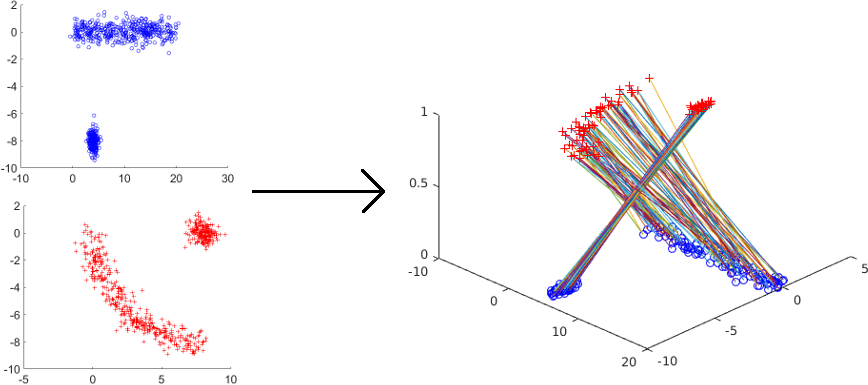
\includegraphics[width = 0.8\textwidth]{./CombinePic/combinepic.png}
  \end{figure}
\end{frame}
% ------------------------------------------------

\begin{frame}
  \frametitle{Change Detection}
  Idea: Compare graph registration against location registration.\\
  Difference in registration $\implies$ change in topology between sets.\\~\\
  With multimodal data, can find what information is portrayed differently between the two sets.
  \begin{figure}[ht]
    \begin{minipage}[b]{0.3\linewidth}
      \centering
      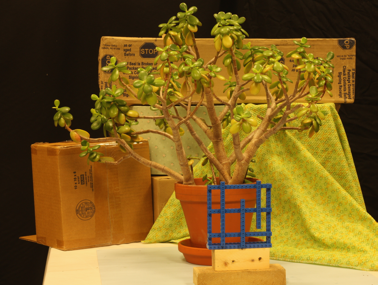
\includegraphics[width=\textwidth]{./JadePlant/pictureX.png}
      \caption{RGB Image}
    \end{minipage}
    \begin{minipage}[b]{0.3\linewidth}
      \centering
      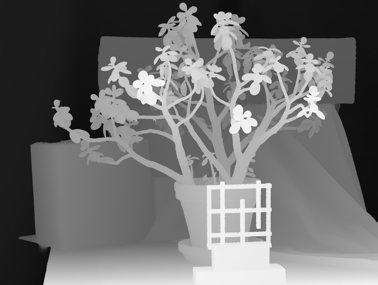
\includegraphics[width=\textwidth]{./JadePlant/pictureY.png}
      \caption{Depth Image}
    \end{minipage}
    \begin{minipage}[b]{0.3\linewidth}
      \centering
      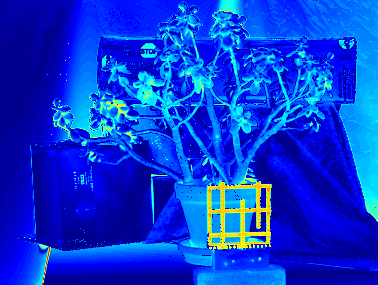
\includegraphics[width=\textwidth]{./JadePlant/ChangesYtoX.png}
      \caption{Change Detection}
    \end{minipage}
  \end{figure}
\end{frame}

% ------------------------------------------------

\end{document}